\section{Main Application Modules}
\label{sec:modules}

\subsection{Module Inventory and Source Code Organization}
The backend architecture is structured around ten core operational modules located across \texttt{backend/app/services/}, \texttt{backend/app/api/routes/}, and \texttt{backend/features/}. 

\begin{figure}[H]
\centering
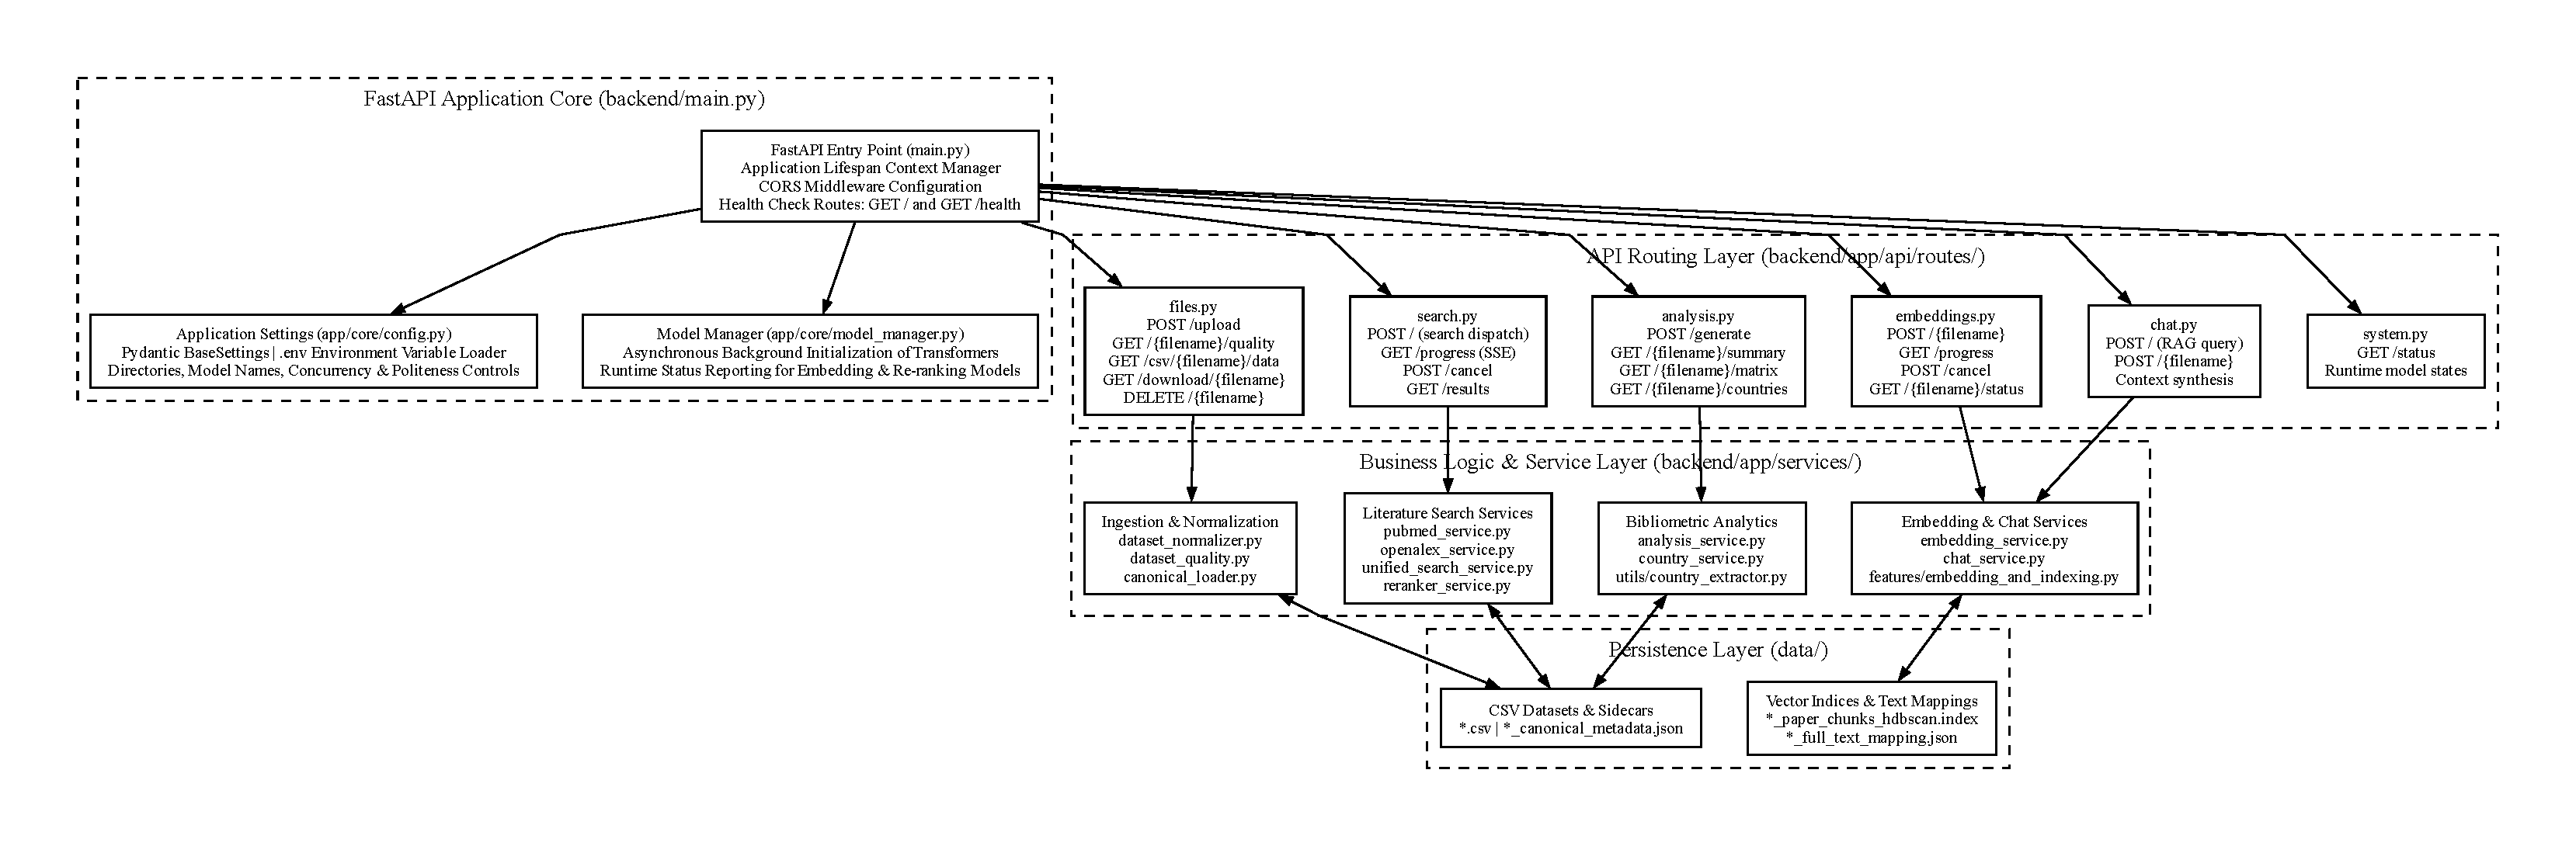
\includegraphics[width=0.92\textwidth]{figures/backend_architecture.pdf}
\caption{Detailed Internal Architecture and Subsystem Interactions of the Backend}
\label{fig:backend_architecture}
\end{figure}

Figure~\ref{fig:backend_architecture} illustrates the routing, service orchestration, and data access flow within the backend.

\subsection{Detailed Technical Description of Modules}

\subsubsection{1. Research Paper Search Module}
\textbf{Files:} \texttt{app/services/search\_service.py}, \texttt{app/api/routes/search.py}\\
Coordinates literature retrieval requests. Supports asynchronous job execution, real-time stage progress reporting via Server-Sent Events (SSE), query cancellation, and export of search results to timestamped CSV files.

\subsubsection{2. PubMed Integration Module}
\textbf{Files:} \texttt{app/services/pubmed\_service.py}, \texttt{app/services/pubmed\_affiliation\_enricher.py}\\
Interfaces directly with NCBI E-utilities. Performs query translation, abbreviation expansion, XML response parsing, author list parsing, MeSH term extraction, and affiliation country resolution.

\subsubsection{3. OpenAlex Integration Module}
\textbf{Files:} \texttt{app/services/openalex\_service.py}\\
Queries the OpenAlex API to fetch multidisciplinary scholarly literature. Handles pagination, DOI normalization, citation counts, concept tags, and institutional affiliation mapping.

\subsubsection{4. Unified Search and Re-ranking Module}
\textbf{Files:} \texttt{app/services/unified\_search\_service.py}, \texttt{app/services/reranker_service.py}\\
Enables simultaneous federated querying across PubMed and OpenAlex with result deduplication based on normalized DOIs. Incorporates NCBI's MedCPT bi-encoder models (\texttt{MedCPT-Query-Encoder} and \texttt{MedCPT-Article-Encoder}) to re-score candidate manuscripts against the search query, placing semantically relevant papers at the top of the result list.

\subsubsection{5. Keyword Analysis Module}
\textbf{Files:} \texttt{app/services/analysis\_service.py}, \texttt{app/api/routes/analysis.py}\\
Performs natural language tokenization, lemmatization, and stop-word filtering across research titles, abstracts, and author keywords. Computes term frequency distributions and outputs \texttt{*\_analysis\_keyword\_frequency.csv}.

\subsubsection{6. Keyword Co-occurrence Analysis Module}
\textbf{Files:} \texttt{app/services/analysis\_service.py}\\
Constructs symmetric co-occurrence presence matrices measuring the pairwise frequency with which research concepts appear within the same manuscript. Generates \texttt{*\_analysis\_keyword\_presence\_matrix.csv} for cluster analysis and thematic mapping.

\subsubsection{7. Country Collaboration Analysis Module}
\textbf{Files:} \texttt{app/services/country\_service.py}, \texttt{app/utils/country\_extractor.py}\\
Parses author affiliation text strings using regular expressions and international country dictionaries. Builds undirected collaboration network graphs where nodes represent sovereign nations and edge weights quantify co-authored publications. Produces telemetry for interactive 2D and 3D globe visualizations.

\subsubsection{8. AI Research Assistant (RAG) Module}
\textbf{Files:} \texttt{app/services/chat\_service.py}, \texttt{app/api/routes/chat.py}\\
Implements an advanced Retrieval-Augmented Generation (RAG) conversational pipeline. Complex user queries are decomposed into targeted sub-queries, evaluated against the FAISS dense vector store, deduplicated, and formatted into an evidence context passed to Google Gemini (\texttt{gemini-2.5-flash}) with instructions to generate cited answers.

\subsubsection{9. Embedding and Vector Indexing Module}
\textbf{Files:} \texttt{app/services/embedding\_service.py}, \texttt{features/embedding\_and\_indexing.py}\\
Manages dense representation pipelines. Chunks manuscript texts into 512-token segments with 50-token overlap, encodes chunks into 768-dimensional dense vectors using \texttt{all-mpnet-base-v2}, and serializes the resulting index to disk in FAISS binary format (\texttt{*\_paper\_chunks\_hdbscan.index}).

\subsubsection{10. Dataset Management and Upload Module}
\textbf{Files:} \texttt{app/api/routes/files.py}, \texttt{app/utils/csv\_loader.py}\\
Handles client-side CSV file uploads, enforces file size constraints ($\le 100$ MB), supports file deletion, serves paginated dataset previews, and provides secure download endpoints for generated analytical assets.
